We now give a synopsis of the proof of soundness of the logic from \S \ref{sect:proofSystem}, and outline the 
 two most interesting aspects: deep satisfaction, and summarized execution.

 
\paragraphSD{\Strong Satisfaction} 
\label{s:scoped:valid}
We are faced with the challenge that assertions are not always preserved when  the top frame is popped (\cf Ex. \ref{ex:pop:does:not:preserve}),  yet we must be able to argue that method return preserves the method body's postconditions.
 For this, we introduce a  ``deeper'' notion of assertion satisfaction, which an assertion be satisfied not only from the perspective of the top frame, but also from the perspective of every frame starting from the $k$-th frame onwards:   $ \satDAssertFrom M  \sigma k   A$   says that   $\forall j. [\  k\!\leq\! j \leq\! \DepthSt \sigma \ \Rightarrow \ M, \RestictTo \sigma j \models A \ ]$.
Accordingly, we introduce \emph{\strong specification satisfaction},  ${\satDAssertQuadrupleFrom \Mtwo  M  \sigma   {A} {A'} {A''} } $, which promises for all $k\!\leq\! \DepthSt \sigma$,  
if $ \satDAssertFrom M  \sigma k   A$, and    if %-- shorter
  scoped execution of $\sigma$'s continuation leads to final state $\sigma'$ and intermediate external state $\sigma''$, then
 $ \satDAssertFrom M  {\sigma'} k   {A'}$, and  $ \satDAssertFrom M  {\sigma''} k   {A''}$
 -  \cf    App.\aref{G.3}{\ref{s:shallow:deep:appendix}}.
 
 Here how \strong satisfaction addresses this problem: Assume    state  $\sigma_1$  right before entering a call, $\sigma_2$ and $\sigma_3$ at start and end of the call's body, and   $\sigma_4$ upon return. If a  pre-condition holds at $\sigma_1$,  then it  holds for a $k\leq \DepthSt {\sigma_1}$; hence,  if the postcondition holds for $k$ at $\sigma_3$, and because $\DepthSt {\sigma_3}= \DepthSt {\sigma_1}\!+\!1$, it also holds for $\sigma_4$.    
% We define   $\satisfiesD {M} {\quadruple  {A} }   {stmt}   {A'} {A''} $ and  $\satisfiesD {M} {S}$ accordingly.
\Strong satisfaction is stronger than shallow (\ie  specification satisfaction as in Def. \ref{def:shallow:spec:sat:state}). 
 
\begin{lemma}% [\Strong  implies  Shallow Satisfaction]
For all $\Mtwo$, $M$, $A$, $A'$, $A''$, $\sigma$:  
\begin{itemize}
\item
 $ {\satDAssertQuadrupleFrom \Mtwo  M  \sigma   {A} {A'} {A''} } \ \Longrightarrow \ \
  {\satAssertQuadruple  \Mtwo  M   {A}  \sigma  {A'} {A''} } $\end{itemize}
\end{lemma}


\paragraphSD{Soundness of the Triples Logic}
\label{sect:prove:triples:sound}
We require the assertion logic,  $M\vdash A$, and  the  underlying Hoare logic,  $M\ \vdash_{ul}\  \triple A {stmt} {A'}$,   to be be  sound. 
Such  sound logics do exist.
Namely, one can build an assertion logic, $M\vdash A$, by extending a logic which does not talk about protection, through the addition of structural rules which talk about protection; this extension preserves soundness - \cf  App. \aref{G.1}{\ref{s:expectations}}. 
Moreover,  since the assertions $A$ and $A'$ in $M \vdash_{ul}\  \triple A {stmt} {A'}$ may, but need not, talk about protection, 
one can take a Hoare logic from the literature as the $ \vdash_{ul}$-logic.

We then prove   soundness of the rules about protection from Fig. \ref{f:protection}, and, based on this, 
we prove soundness of the inference system for triples  -- \cf \A\ \aref{G.5}{\ref{s:sound:app:triples}}.

 

\begin{Theorem}
\label{l:triples:sound}
For module  $M$   such that  $\vdash M$, and for any assertions $A$,  $A'$, $A''$ and statement  $stmt$:
\begin{center}
$M\ \vdash\  \triple A {stmt} {A'}  \ \ \ \  \Longrightarrow  \ \ \ \ \satisfiesD {M} {\quadruple {A} {stmt} {A'} {A''}}$
\end{center}
\end{Theorem}
 

\paragraphSD{Summarised Execution}
\label{s:summaized}
%Soundness of   rule {\sc{Call\_Ext}} raises the challenge that 
Execution of an external call may consist of any number of external
transitions, interleaved with calls to public internal methods, which in
turn may make any number of further internal calls (public or private),  % chopped ``whether'' so as to be more succinct
and these, again may call external methods.
For the   proof of soundness,  internal and external transitions use different arguments.
 For  external transitions we consider small steps  and  argue in terms of  preservation of  encapsulated properties,
while for internal calls, we use large steps, and appeal to the method's specification.
Therefore, we define  \emph{sumarized} executions, where  internal calls are collapsed into one, large step, \eg below:
  

\label{sect:termExecs}


% \vspace{.1cm}

\begin{tabular}{lll}
\begin{minipage}{.41\textwidth}
%Original execution %, \textbf{three}  internal \& {four} external calls. 
% 
 \resizebox{4.1cm}{!}{
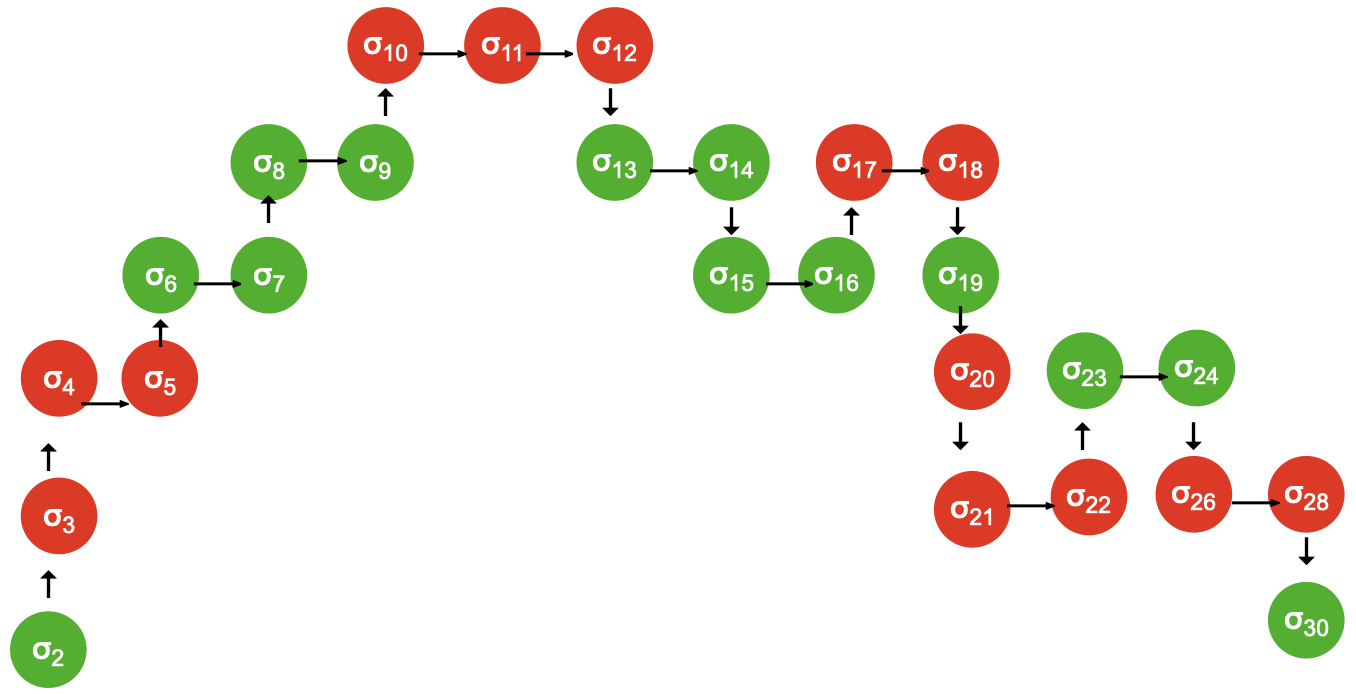
\includegraphics[width=\linewidth]{diagrams/summaryA.png}
} 
 \end{minipage}
&  \begin{minipage}{.14\textwidth}
summarized\\
$\strut \ \ \ \ \ $ to 
\end{minipage}
 &
\begin{minipage}{.41\textwidth}
~ \\
~ \\
\resizebox{4.1cm}{!}
{
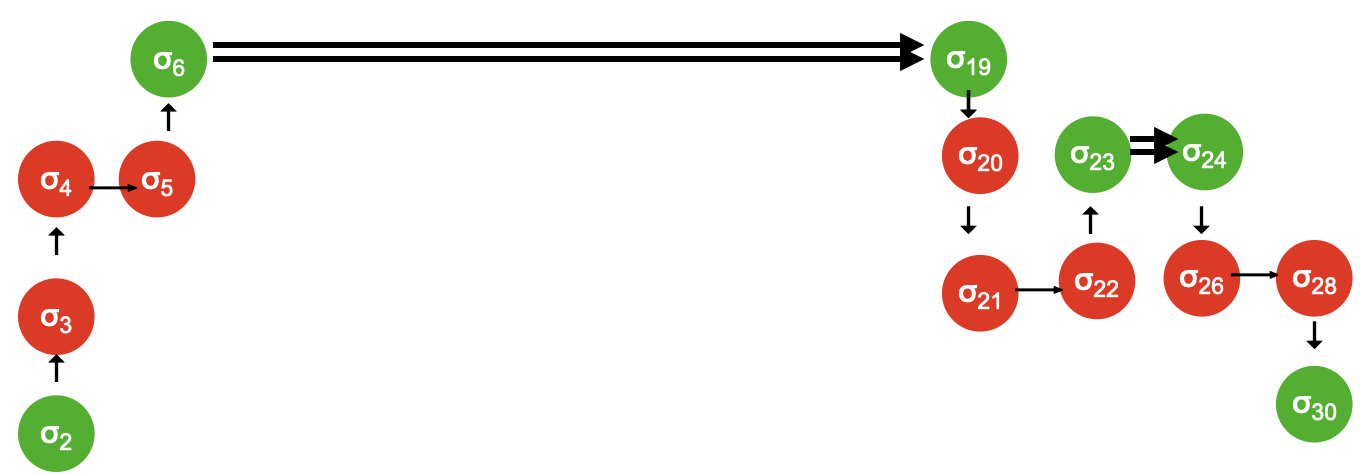
\includegraphics[width=\linewidth]{diagrams/summaryB.png}
} \end{minipage}
\end{tabular}
 
 


\vspace{.05cm}

% We now revisit external executions interleaved with public method calls:   
%In the appendix, we prove 
Lemma \aref{G.28}{\ref{lemma:external_breakdown:term}} % from  the  Appendix   
says that any terminating execution 
 starting in an external state  consists of a  sequence of  external states interleaved with terminating executions
  of public methods.
Lemma  \aref{G.29}{ \ref{lemma:external_exec_preserves_more}} says that such an execution preserves an encapsulated assertion $A$  
provided that all these finalising internal executions  %(the public methods called at $\sigma_1$, ... $\sigma_n$) 
also preserve $A$.
% It is used to prove  soundness of the rule {\sc{ExtCall}}\footnoteSD{perhaps also {\sc{ExtCall\_WithSpec\_Strong}}}
% 
%In the appendix we prove lemmas \ref{lemma:external_breakdown:term} and \ref{lemma:external_exec_preserves_more} 
%which guarantee  that if $\sigma$ is external and $ \leadstoBoundedStarFin {\Mtwo}  {\sigma}  {\sigma'}$, 
%then there exist $\sigma_1$, ... $\sigma_n$, such that
% $\WithExtPub {\Mtwo\cdot M} {\sigma\bd}  {\sigma}  {\sigma'} {\sigma_1...\sigma_n}$.
% Conversely, if $A$ is encapsulated, 
% and $\WithExtPub {\Mtwo\cdot M} {\sigma\bd}  {\sigma}  {\sigma'} {\sigma_1...\sigma_n}$, and 
% the calls at  $\sigma_1$, ... $\sigma_n$ preserve $A$,  then $A$ is preserved from $\sigma$ to $\sigma'$.
  


  %%%%%%%%%%%%%%%%%%%%%%%%%%%%%%%%%%%%%%%%%%%%%%%%%%%

\paragraphSD{ Soundness of the Quadruples Logic}
Proving soundness of our quadruples  requires  induction on the execution  in  some cases, and  induction on the derivation of the quadruples in others.  We address this   through  a well-founded ordering that combines both, \cf 
\label{sect:prove:wellfounded}
\label{sect:prove:sound:quadruples}
  Def.  \aref{G.22}{\ref{def:measure}}  and  Lemma \aref{G.23}{\ref{lemma:normal:two}}. 
  Finally, in \S \aref{G.16}{\ref{s:app:proof:sketch;quadruples}}, we prove soundness:
 

\begin{theorem}
\label{t:quadruple:sound}
\label{thm:soundness}
For module  $M$,   assertions $A$, $A'$, $A''$,   state  $\sigma$, and specification $S$:

\begin{enumerate}[(A)]
\item
 $:\strut \   \vdash M  \ \ \ \wedge \ \ \  M\ \vdash\  \quadruple {A} {stmt} {A'} {A''}  \ \ \ \ \ \ \ \Longrightarrow \ \ \ \ \ \  \ \ \  M\ \modelsD\  \quadruple {A} {stmt} {A'} {A''}$
 \item
  $:\strut \  \  \proves{M}{S}\ \ \ \ \ \ \Longrightarrow\ \ \ \ \ \  \ \ \ {M} \modelsD {S}$
 
\end{enumerate}

\end{theorem}

%The proofs make use of summarized executions, well-founded orderings, and various assertion preservation properties.  %
%\begin{theorem}[Soundness]
%\label{thm:soundness}
%%Assume an \SpecO proof system, $\proves{M}{A}$, 
%%an encapsulation inference system, $\proves{M}{\encaps{A}}$,
%%% Axiom xx, and 
%% and  that on top of these systems we built
%% the \SpecLang logic according to zzzz,  then, for    all modules $M$, and all \SpecLang specifications  $S$:
% For any module $M$, and specification $S$:
% 
% $$\proves{M}{S}\ \ \ \ \ \ \ \mbox{implies}\ \ \ \ \ \  \ \ \ {M} \modelsD {S}$$
%\end{theorem}
%
%We now prove soundness of the inference system $M \vdash  \quadruple A {stmt} {A'} {A''}$, using summarized executions from the earlier section, and the ordering $_ \ll \_$:   Proof outlines for these theorems can be found in \A \ref{s:app:proof:sketch;quadruples} and \ref{s:app:proof:sketch;overall}. 

%
%Theorem. \ref{thm:soundness} demonstrates 
% that the   \SpecLang logic is sound with respect to the semantics of \SpecLang specifications.
% The \SpecLang logic parametric wrt to the algorithms for proving validity of assertions
% $\proves{M}{A}$, and 
% assertion encapsulation ($\proves{M}{\encaps{A}}$), and is sound
% provided that these two proof systems are sound.
